
\documentclass[14pt]{extarticle}
\usepackage{graphicx}
\usepackage{pdfpages}
\usepackage[T1]{fontenc}
\usepackage[margin=1in]{geometry}

\graphicspath{ {./images/} }

\begin{document}
    \pagenumbering{arabic}
    \pagestyle{plain}

    \title{\Huge Assignment 4\\ Computer Networks}
    \author{\huge Vikas Gola : 2016UCS0023}
    \maketitle
    \newpage

    \begin{center}
        {\large \textbf{SET 1: The Basic HTTP GET/response interaction }}
    \end{center}


    \begin{center}
        {\large \textmd{Images for first seven questions and captured packets for simple1.html page}}\\
    \end{center}
    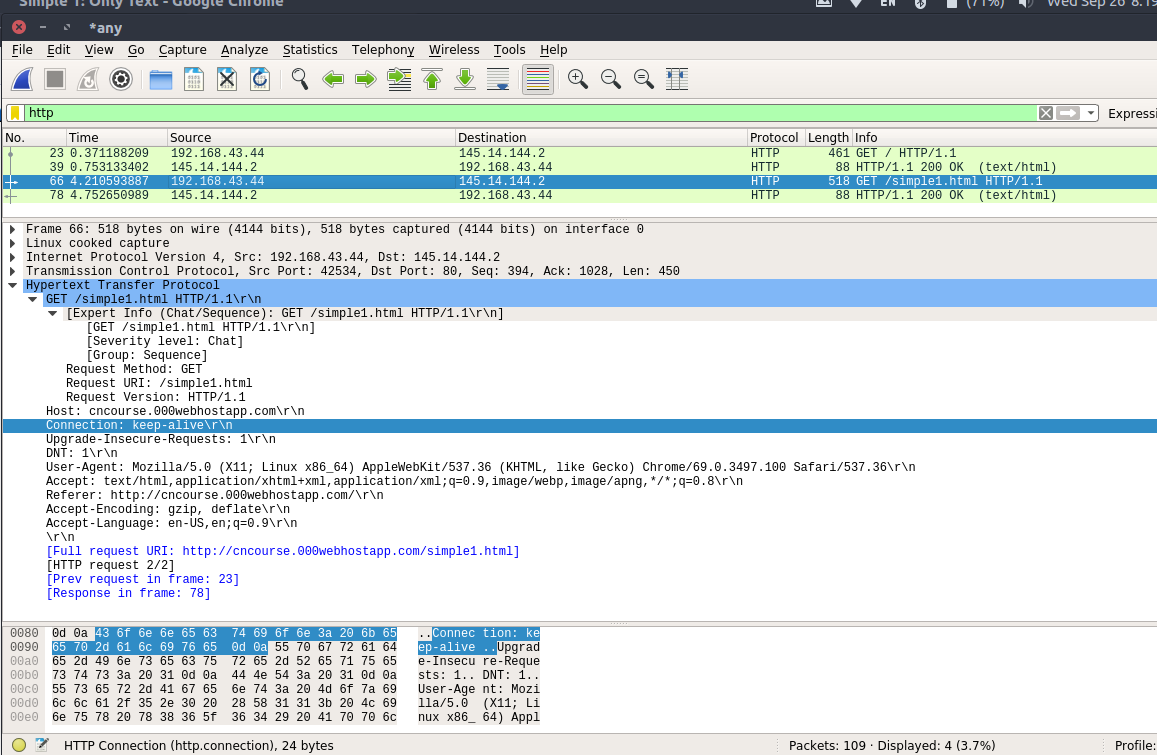
\includegraphics[scale=0.40]{1_1}\\[10pt]
    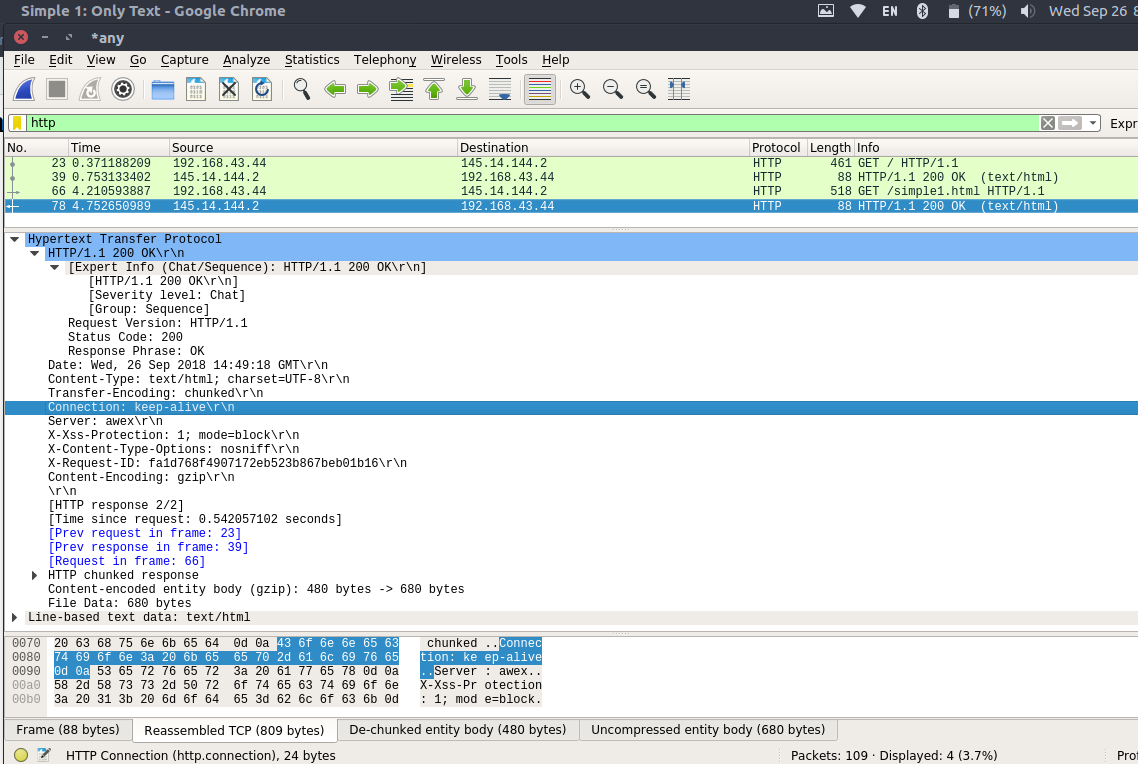
\includegraphics[scale=0.40]{1_2}\\[10pt]

    \noindent
    \textbf{\large Question 1}
    Is your browser running HTTP version 1.0 or 1.1?  What version of HTTP is the server running?\\
    \textbf{\large Answer}
    My browser is running HTTP version 1.1 . Server is also running HTTP version 1.1 .\\
    \vspace{1cm}
    
    \noindent
    \textbf{\large Question 2}
    What languages (if any) does your browser indicate that it can accept to the server?\\
    \textbf{\large Answer}
    My browser can accept en-US, en.\\
    % 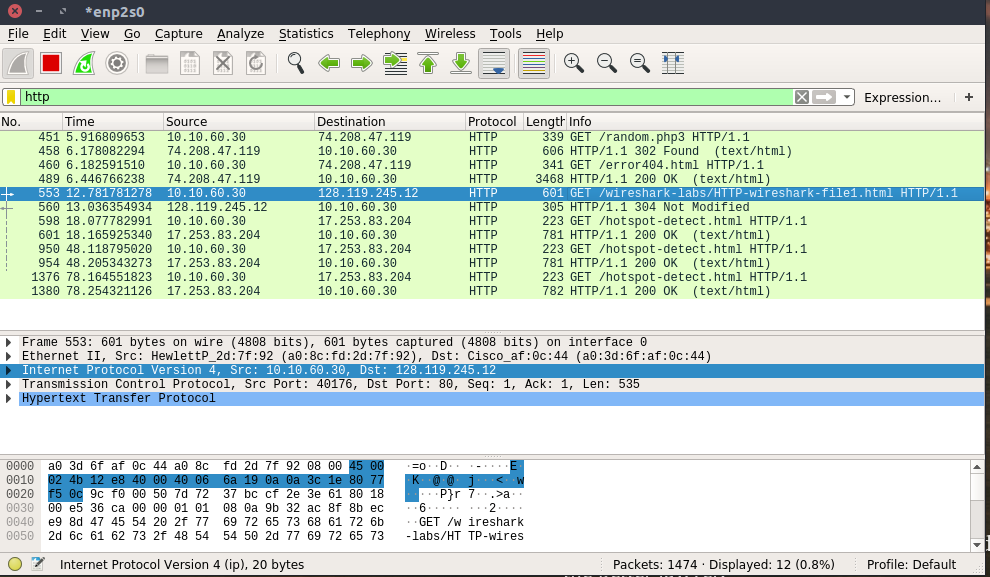
\includegraphics[scale=0.48]{2}
    \vspace{1cm}
    
    \noindent
    \textbf{\large Question 3}
    What is the IP address of your computer?  Of the cncourseweb server?\\
    \textbf{\large Answer}
    IP address of my computer: 192.168.43.44\\
    IP address of server: 145.14.144.2\\
    % 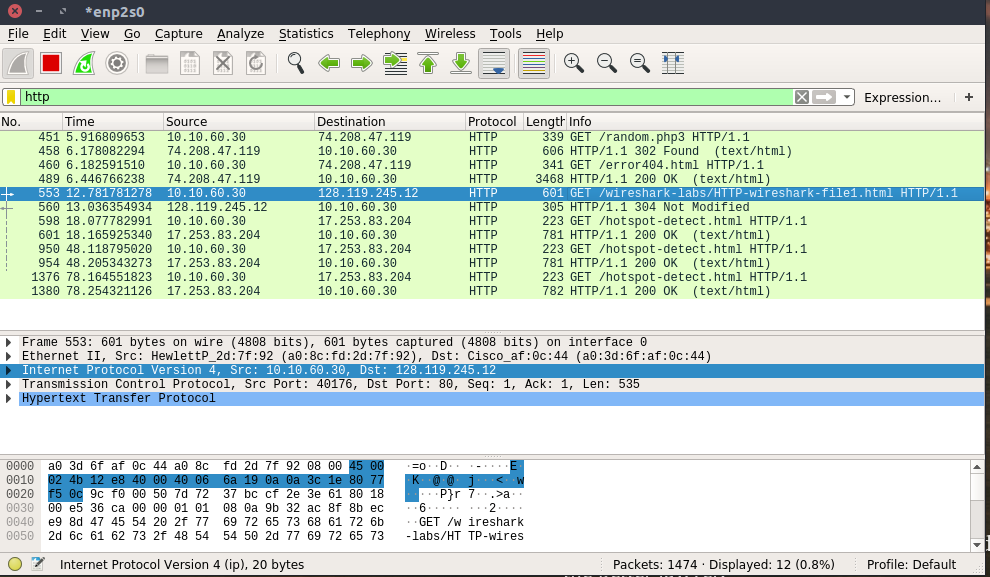
\includegraphics[scale=0.48]{2}
    \vspace{1cm}
    
    \noindent
    \textbf{\large Question 4}
    What is the status code returned from the server to your browser?\\
    \textbf{\large Answer}
    Status Code: 200\\
    % 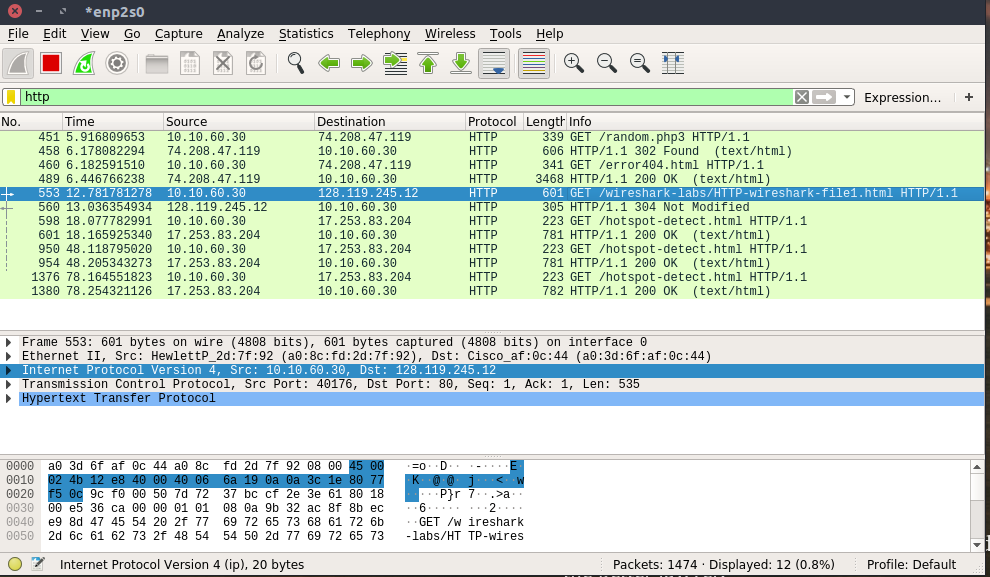
\includegraphics[scale=0.48]{2}
    \vspace{1cm}
    
    \noindent
    \textbf{\large Question 5}
    When was the HTML file that you are retrieving last modified at the server?\\
    \textbf{\large Answer}
    last modified not given in response and can be verified in snapshots.\\
    % 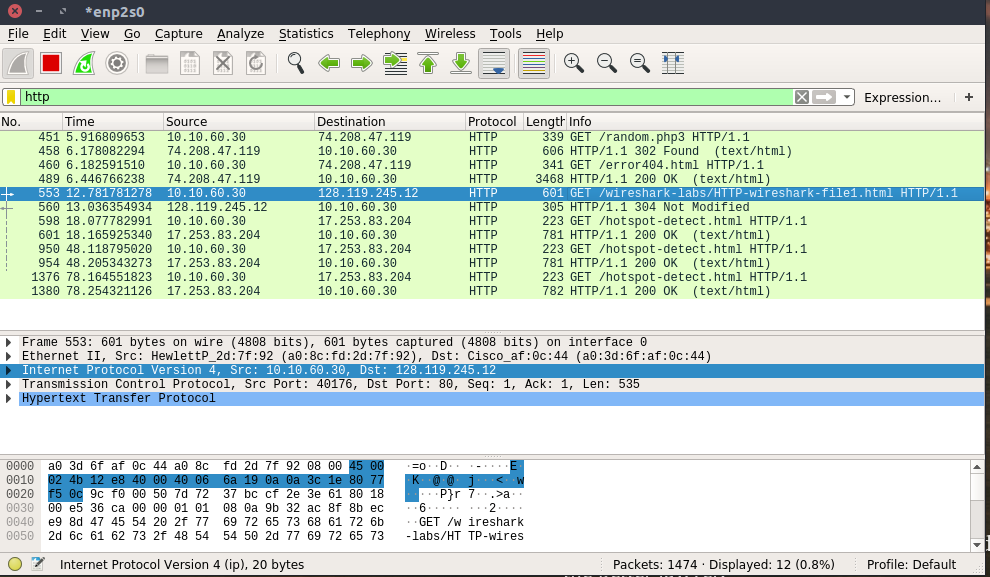
\includegraphics[scale=0.48]{2}
    \vspace{1cm}
    
    \noindent
    \textbf{\large Question 6}
    How many bytes of content are being returned to your browser?\\
    \textbf{\large Answer}
    Content length is not given in response to browser but Bytes length of File data is given which is 680 bytes.\\
    % 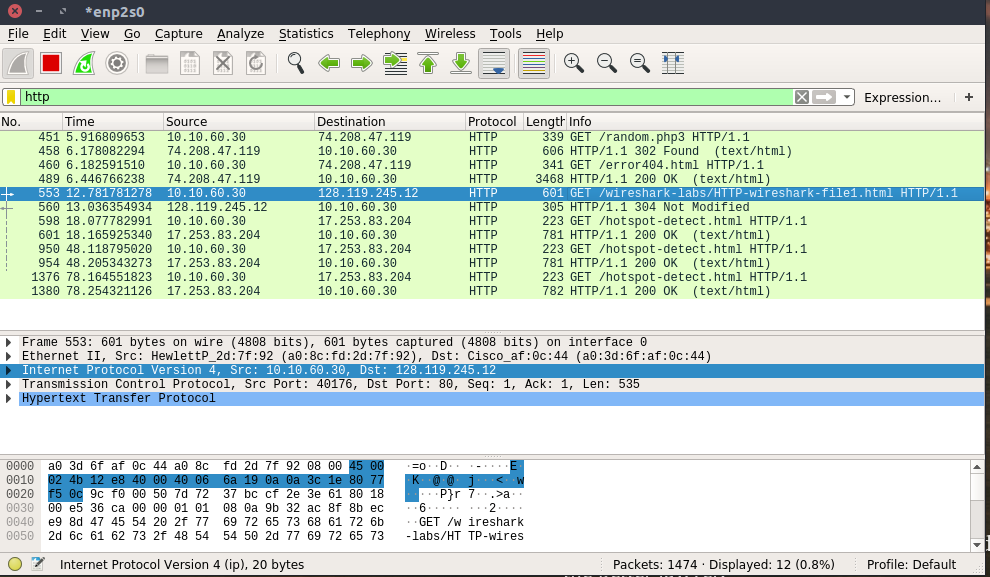
\includegraphics[scale=0.48]{2}
    \vspace{1cm}
    
    \noindent
    \textbf{\large Question 7}
    By inspecting the raw data in the packet content window,
    do you see any headers within the data that are not displayed 
    in the packet-listing window?  If so, name one.\\
    \textbf{\large Answer}
    no, I don't see any in the HTTP Message.\\
    % 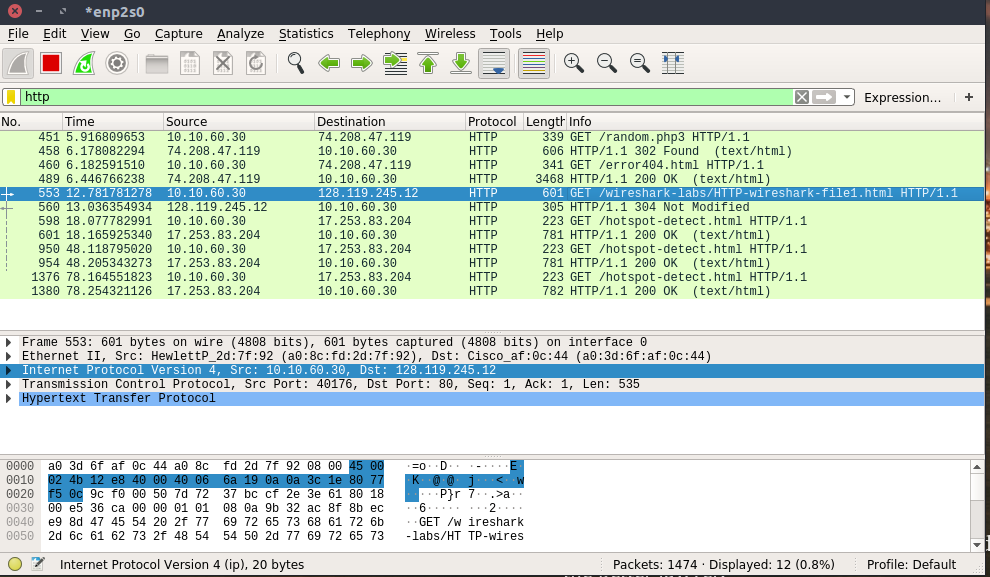
\includegraphics[scale=0.48]{2}
    \vspace{1cm}


    \noindent
    \textbf{\large Question 8}
    Click the following command on Wireshark menu:  Statistics->http->Requests. 
    Find out how many requests were sent by your browser and how many did the server respond, with ?\\
    \textbf{\large Answer}
    2 requests were sent by browser one for index page and second for simple1 page and 2 respond received from the server.\\[10pt]
    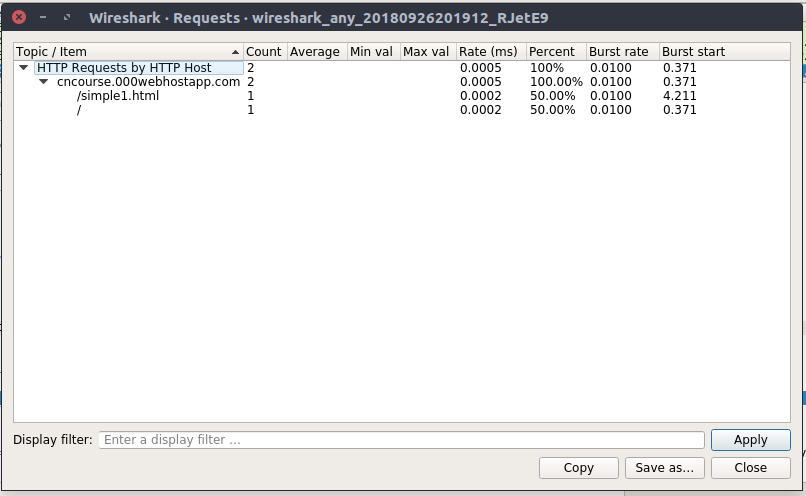
\includegraphics[scale=0.55]{1_4}\\
    \vspace{1cm}
    
    \noindent
    \textbf{\large Question 9}
    Find out how to obtain the http traffic flow graph 
    showing the packet exchanges between the client and the server 
    and take a dump of the flow graph for http packets 
    and paste in your answer sheet after all the questions above are answered.\\
    \textbf{\large Answer}
    To obtain the flow graph go to Statistics->flow graph.Here is flow graph:\\
    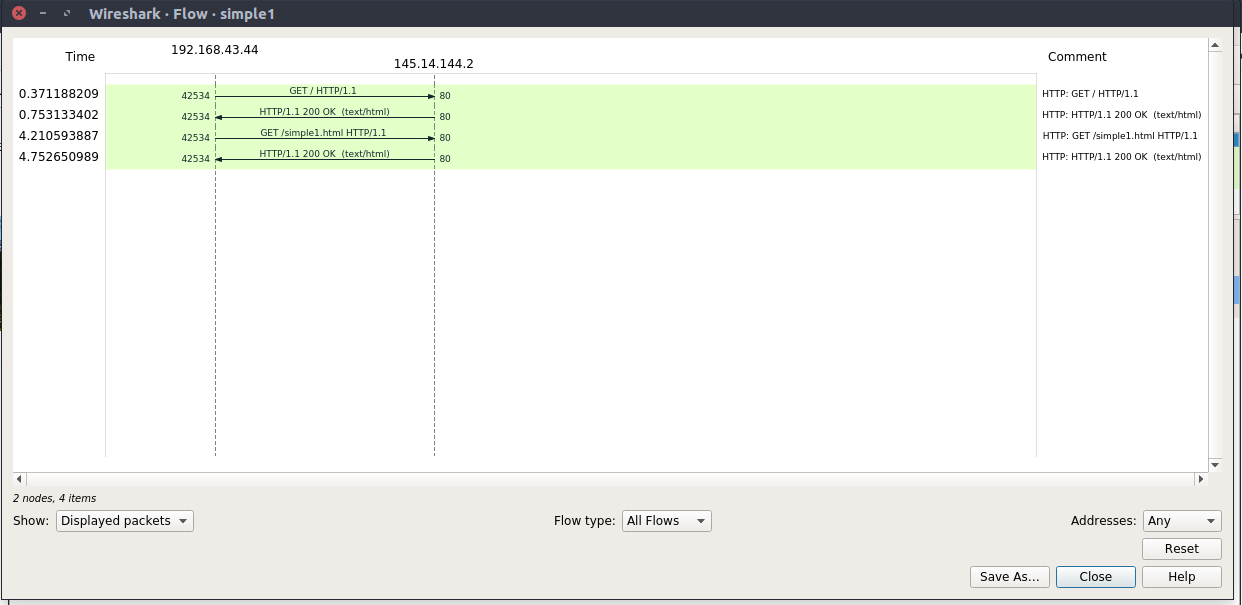
\includegraphics[scale=0.35]{1_5}
    \vspace{1cm}

    \noindent
    \textbf{\large Question 10}
    Now, enter the following URL to your browser, and 
    answer the questions 5,6, 8 and 9 for the following file :
    \textsl{http://cncourse.000webhostapp.com/simple2.html}\\
    \textbf{\large Answer}
    \begin{center}
        {\large \textmd{Images for captured packets for simple2.html page}}\\
    \end{center}
    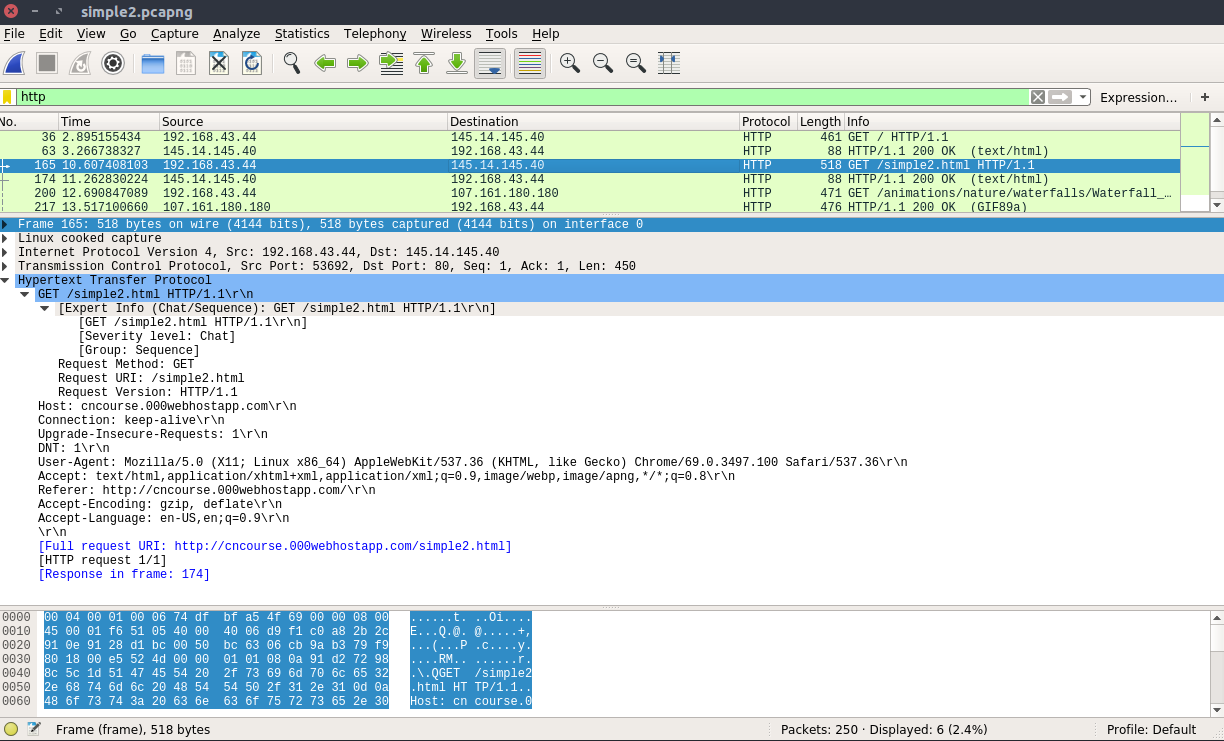
\includegraphics[scale=0.40]{1_10_1}\\[10pt]
    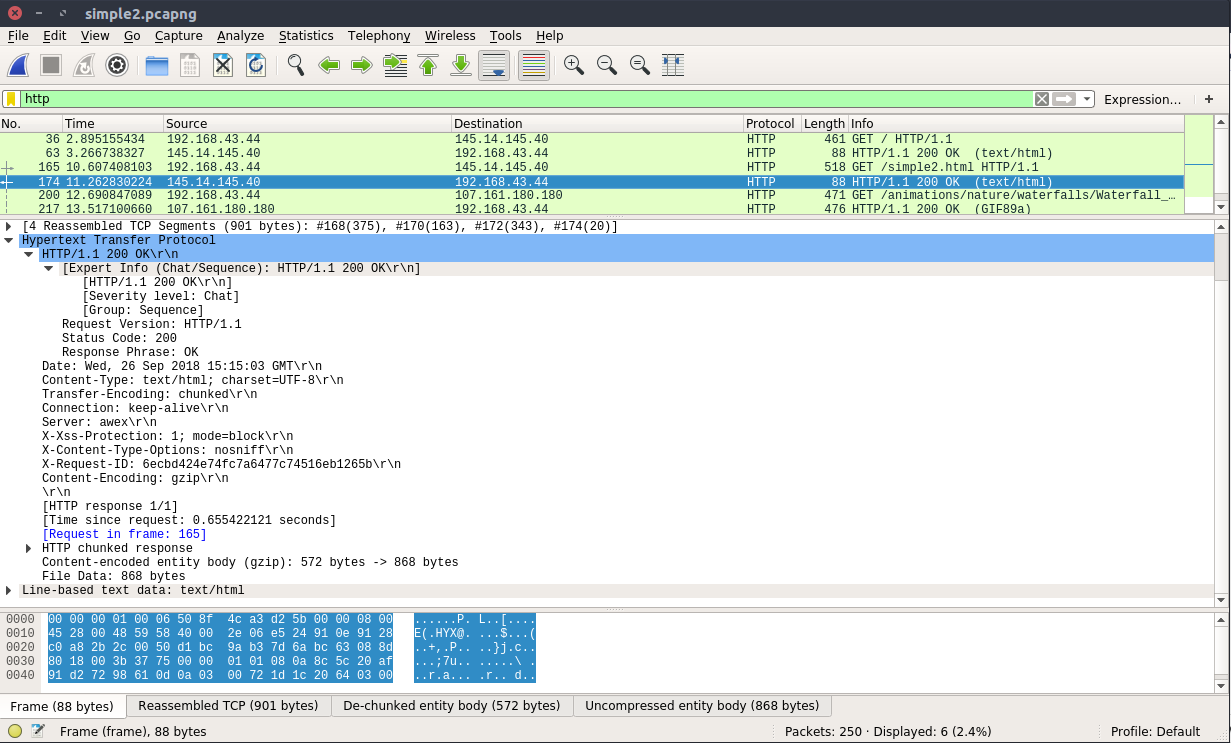
\includegraphics[scale=0.40]{1_10_2}\\[10pt]
    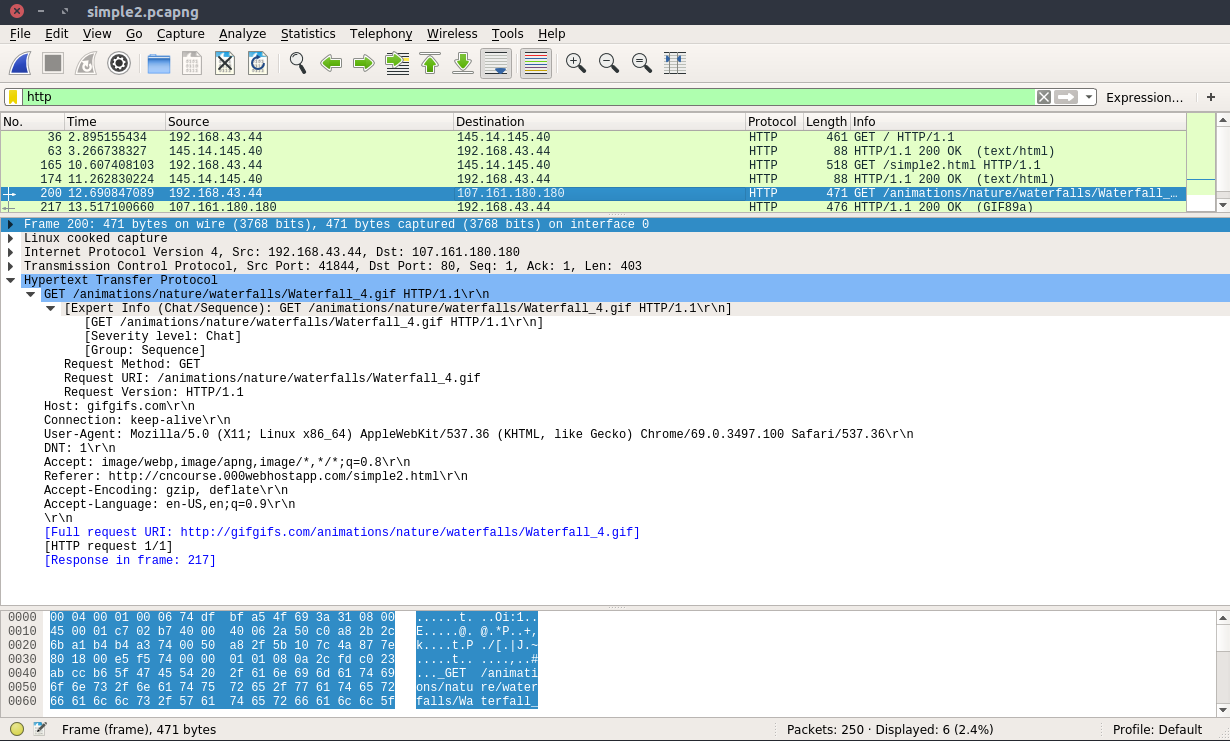
\includegraphics[scale=0.40]{1_10_3}\\[10pt]
    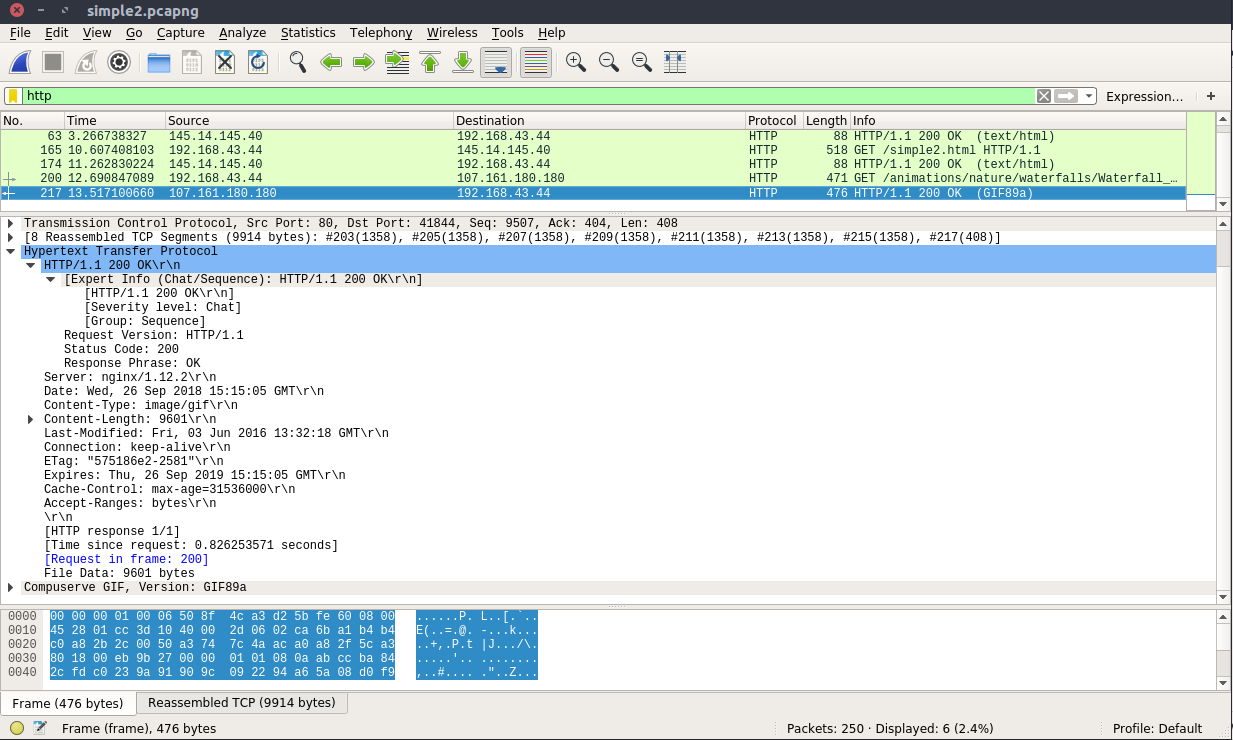
\includegraphics[scale=0.40]{1_10_4}\\[10pt]
    \begin{itemize}
        \item \textbf{Ans 5:} last modified not given in response and can be verified in snapshots.
        \item \textbf{Ans 6:} File Data: 868 bytes(/simple2.html) + 9601 bytes(of gif)
        \item \textbf{Ans 8:} 3 requests(1 for index page, 1 for simple2.html and one for gif)\\[10pt]
        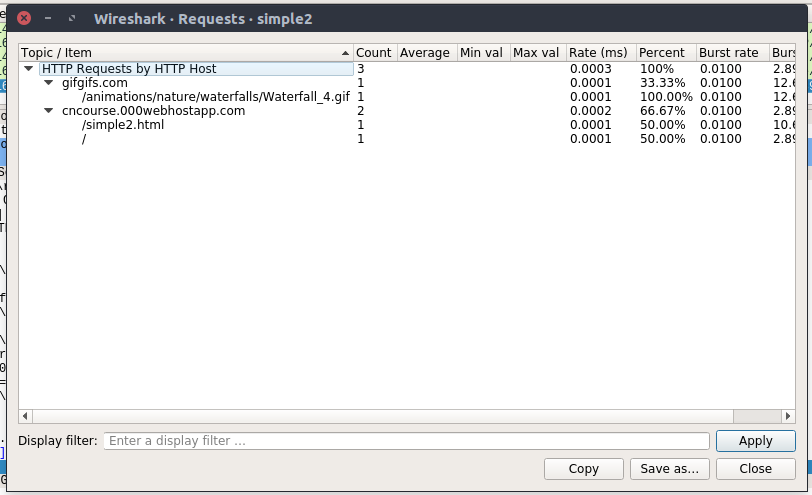
\includegraphics[scale=0.40]{1_10_5}\\[10pt]
        \item \textbf{Ans 9:} Here is flow graph:\\[10pt]
        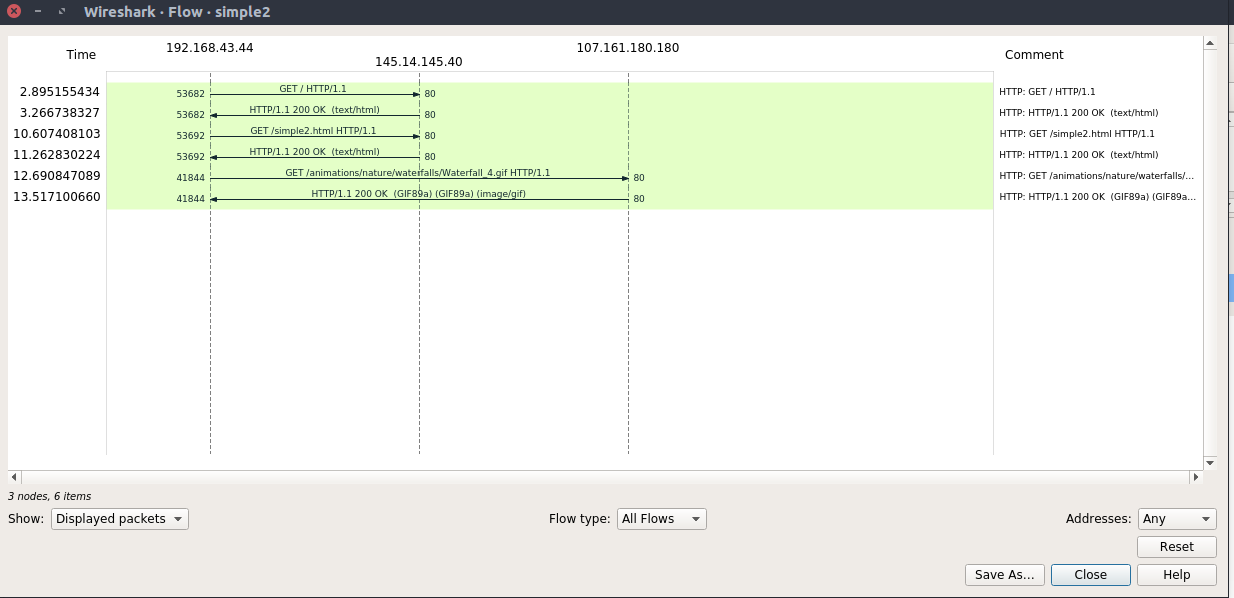
\includegraphics[scale=0.36]{1_10_6}\\[10pt]
    \end{itemize}
    \vspace{1cm}

    \noindent
    \textbf{\large Question 11}
    Now, enter the following URL to your browser, and 
    answer the questions 5,6, 8 and 9 for the following file :
    \textsl{http://cncourse.000webhostapp.com/simple3.html}\\
    \textbf{\large Answer}
    \begin{center}
        {\large \textmd{Images for captured packets for simple3.html page}}\\
    \end{center}
    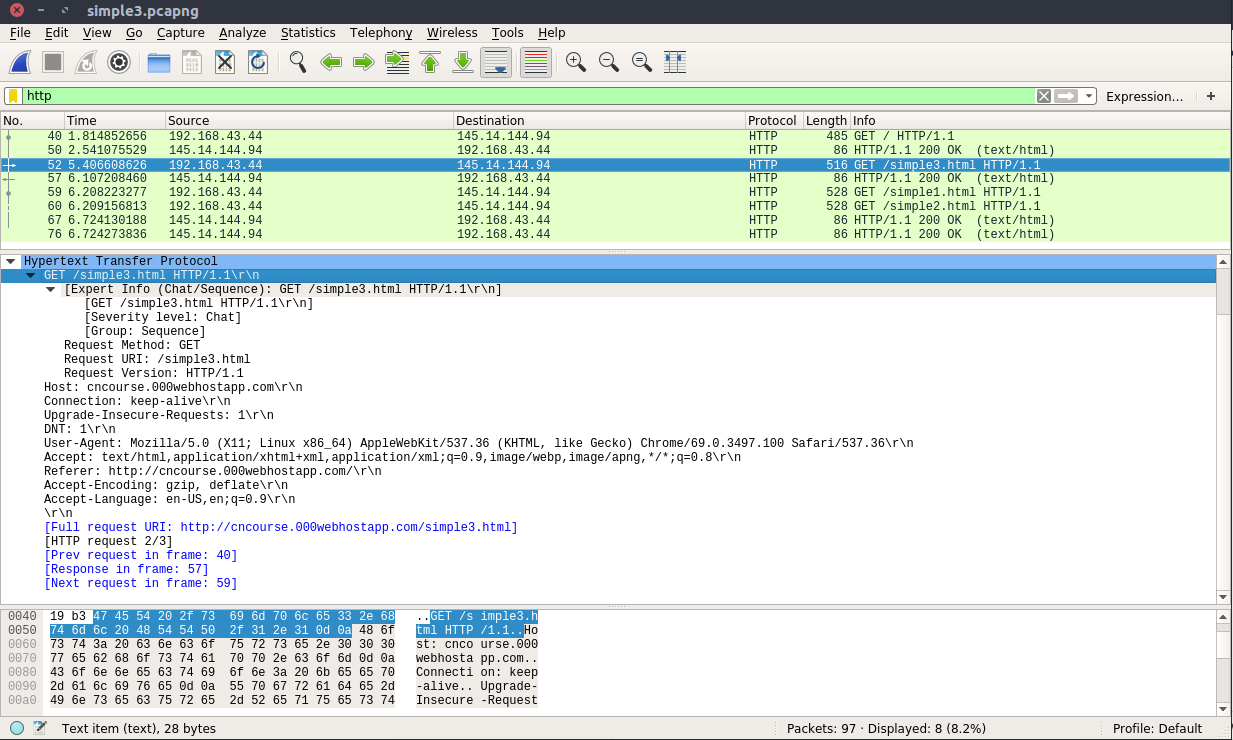
\includegraphics[scale=0.40]{1_11_1}\\[10pt]
    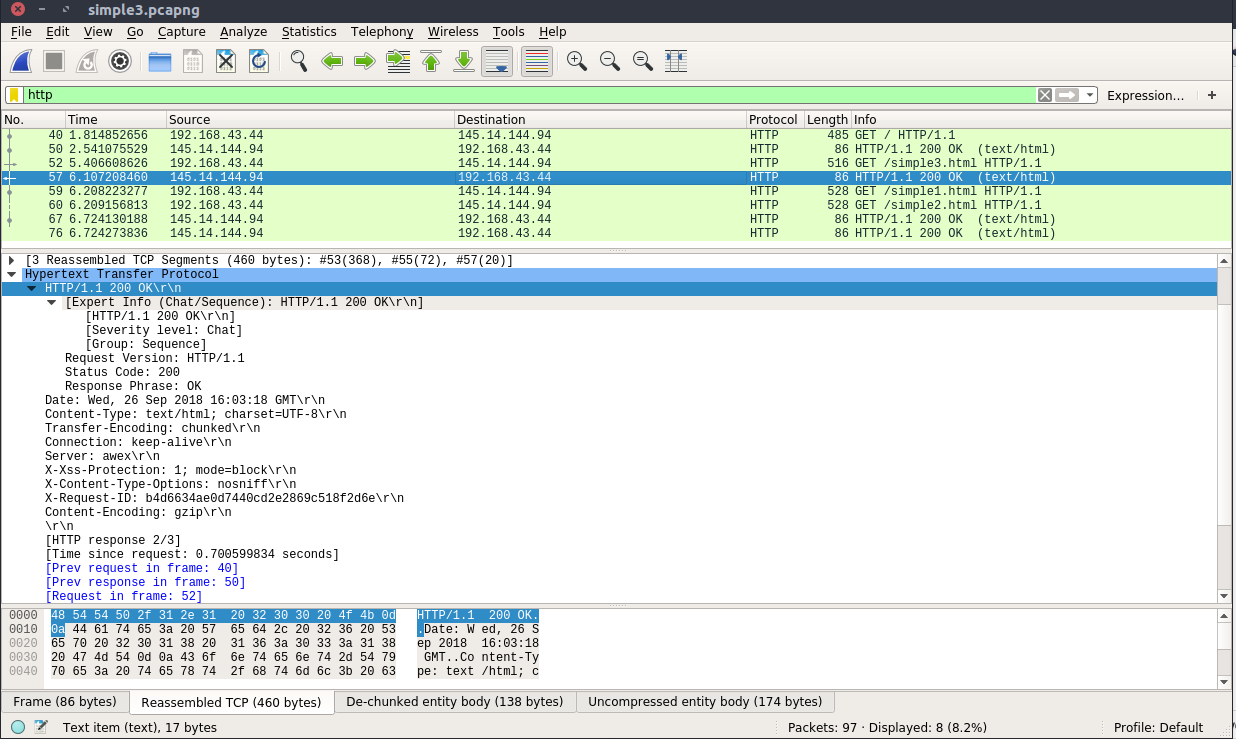
\includegraphics[scale=0.40]{1_11_2}\\[10pt]
    \begin{itemize}
        \item \textbf{Ans 5:} last modified not given in response and can be verified in snapshots.
        \item \textbf{Ans 6:} File Data: 174 bytes(/simple3.html) + 680 bytes(for /simple1.html) + 868 bytes(for /simple2.html)
        \item \textbf{Ans 8:} 4 requests(1 for index page, 1 for simple2.html,1 for simple1.html and 1 for simple3.html )\\[10pt]
        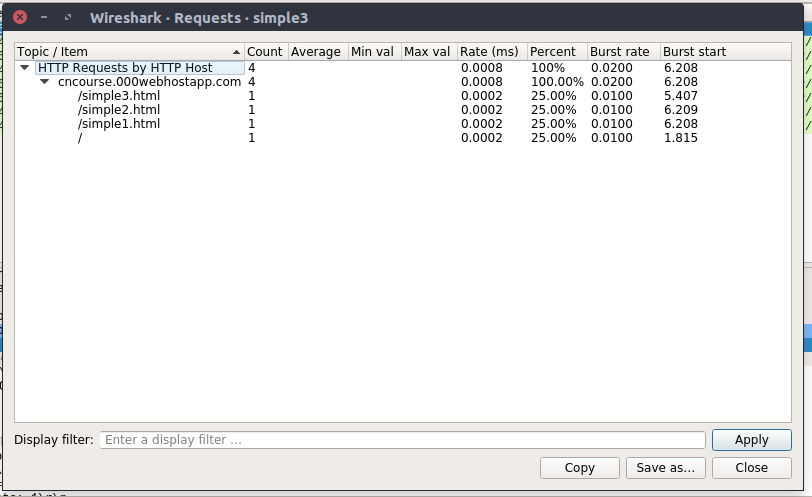
\includegraphics[scale=0.40]{1_11_3}\\[10pt]
        \item \textbf{Ans 9:} Here is flow graph:\\[10pt]
        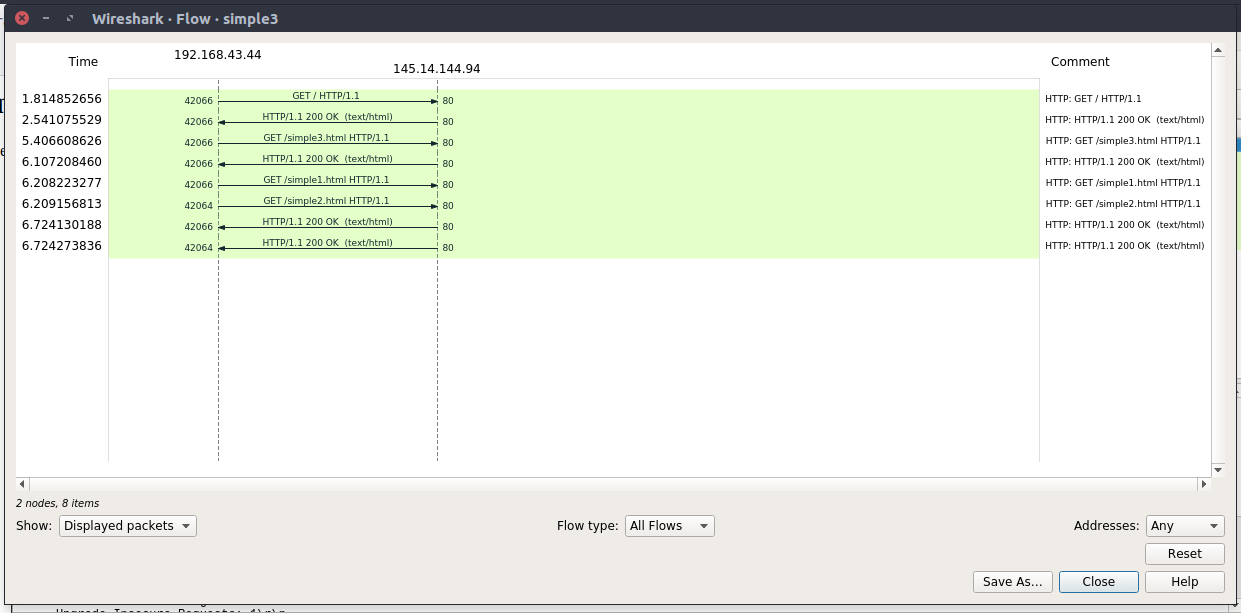
\includegraphics[scale=0.40]{1_11_4}\\[10pt]
    \end{itemize}
    \vspace{1cm}

    \noindent
    \textbf{\large Question 12}
    Now, enter the following URL to your browser, and 
    answer the questions 5,6, 8 and 9 for the following file :
    \textsl{http://cncourse.000webhostapp.com/simple4.html}. Can you tell whether your browser downloaded the ten images serially, or 
    whether they were downloaded from the two web sites in parallel? Explain?\\
    \textbf{\large Answer}
    \begin{center}
        {\large \textmd{Images for captured packets for simple4.html page}}\\
    \end{center}
    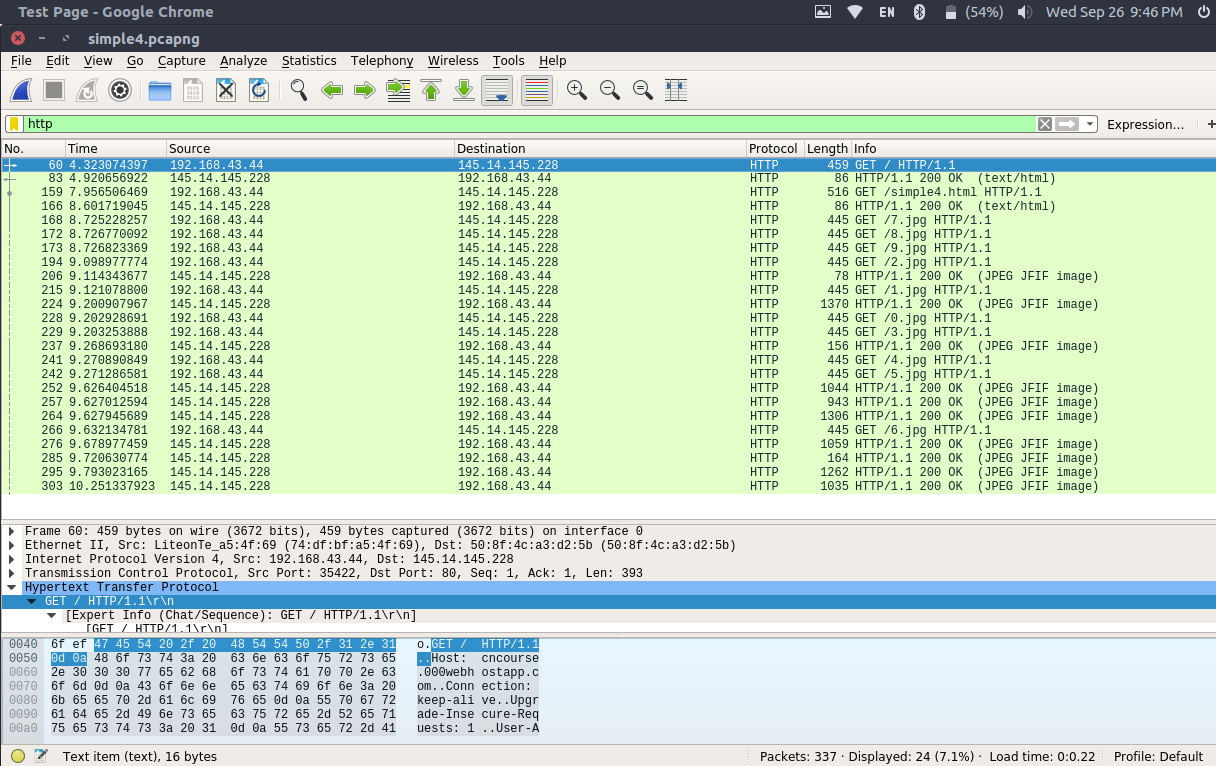
\includegraphics[scale=0.40]{1_12}\\[10pt]
    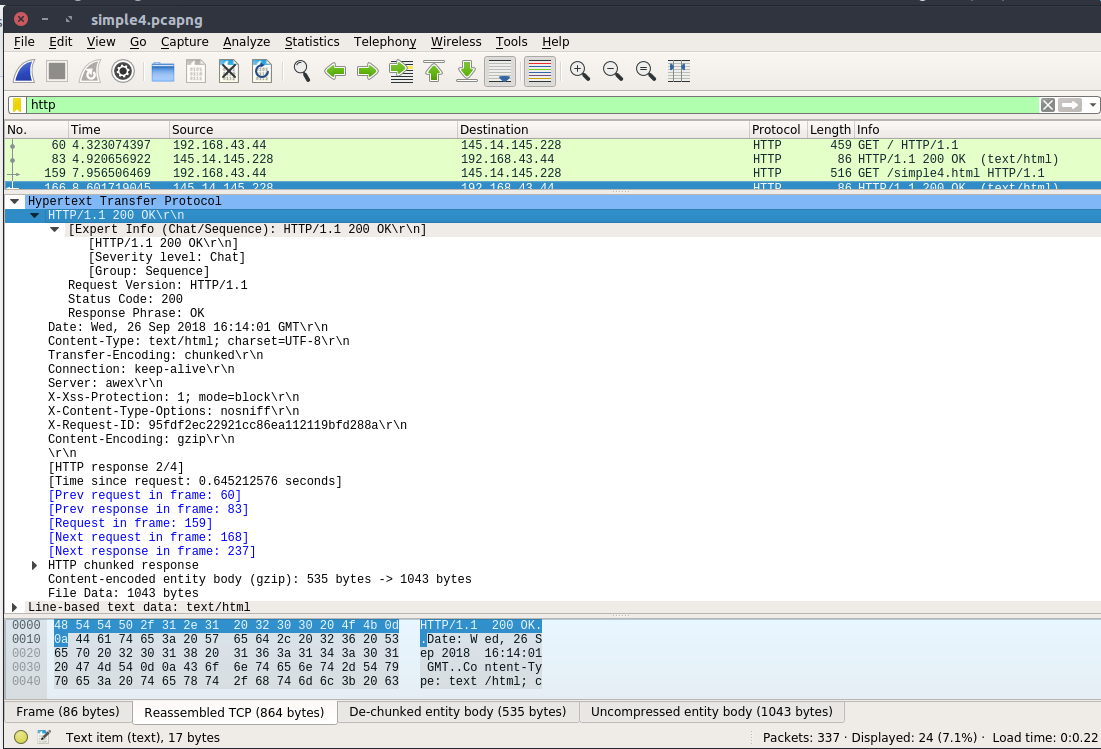
\includegraphics[scale=0.40]{1_12_1}\\[10pt]
    \begin{itemize}
        \item \textbf{Ans 5:} last modified not given in response and can be verified in snapshots.
        \item \textbf{Ans 6:} File Data: 1043 bytes(/simple4.html) + (5259+5193+3840+4867+3269+5129+4882+3987+5085+4858) bytes(of 10 images)
        \item \textbf{Ans 8:} 12 requests(1 for index page, 1 for simple4.html,10 for images of 0 to 9 )\\[10pt]
        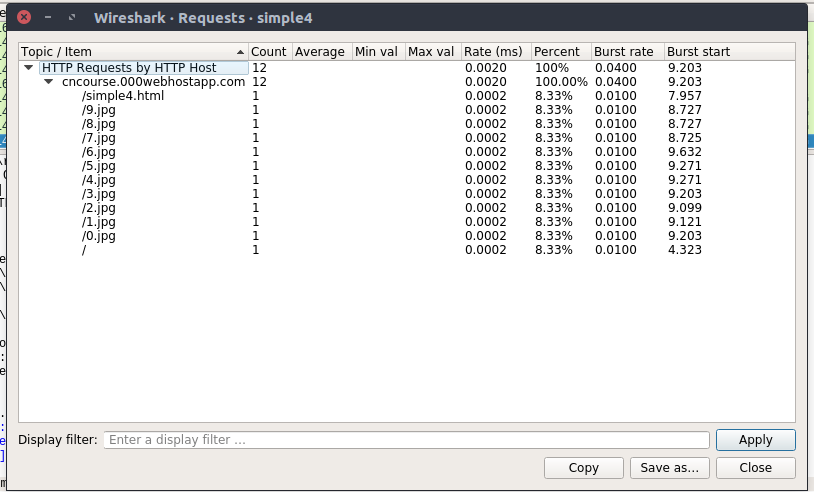
\includegraphics[scale=0.40]{1_12_2}\\[10pt]
        \item \textbf{Ans 9:} Here is flow graph:\\[10pt]
        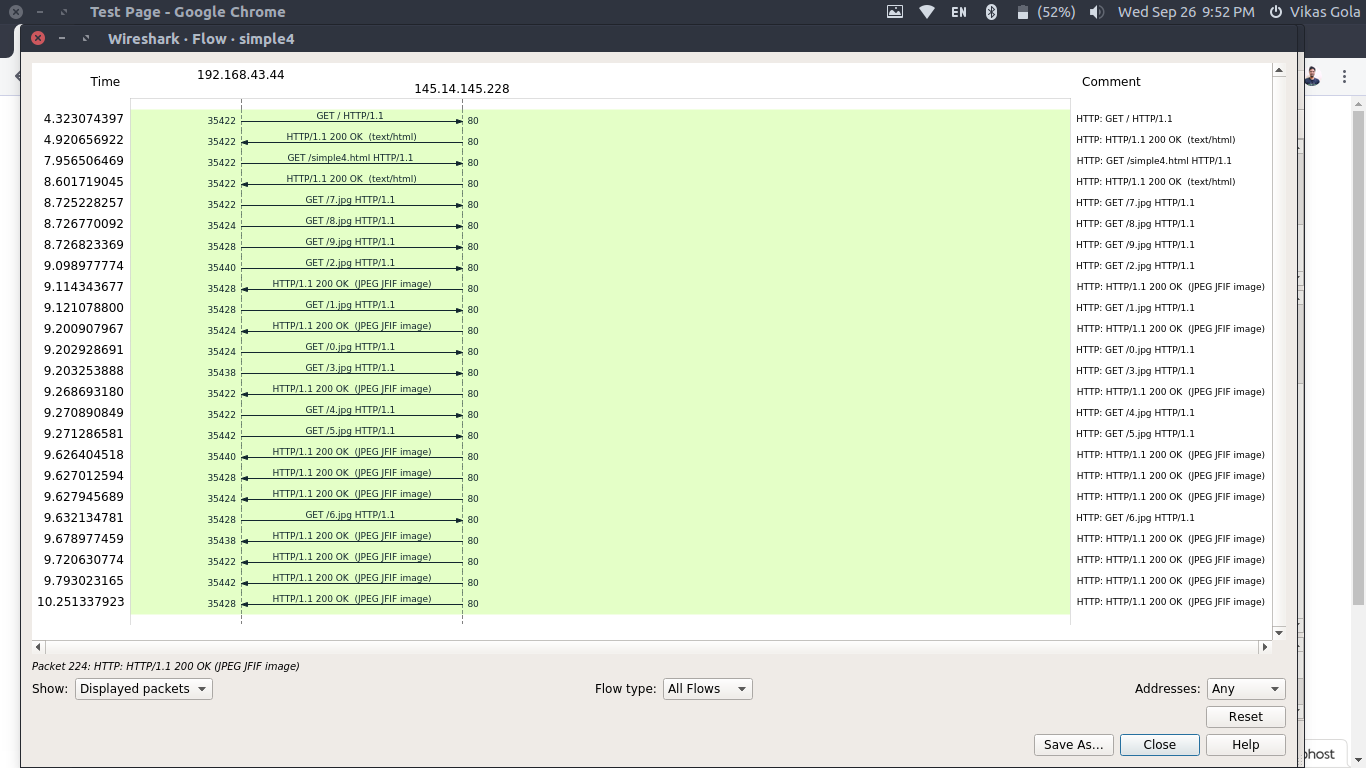
\includegraphics[scale=0.32]{1_12_4}\\[10pt]
    \end{itemize}
    My browser downloaded the images in parallel as images has been requested continuously without for wait to download 
    or get the first image which have been requested first.\\
    \vspace{1cm}

    \noindent
    \textbf{\large Question 13}
    Now, enter the following URL to your browser: 
    {http://www.iitsystem.ac.in/sites/default/files/councilminutes/minutes/51/Revised\_Minutes\_51st\_Meeting\_of\_the\_IITCouncil\_28.4.2017.PDF}. 
    Find the time required to access this file.\\
    \textbf{\large Answer}
    Time Required to access the file = 0.517282393\\[10pt]
    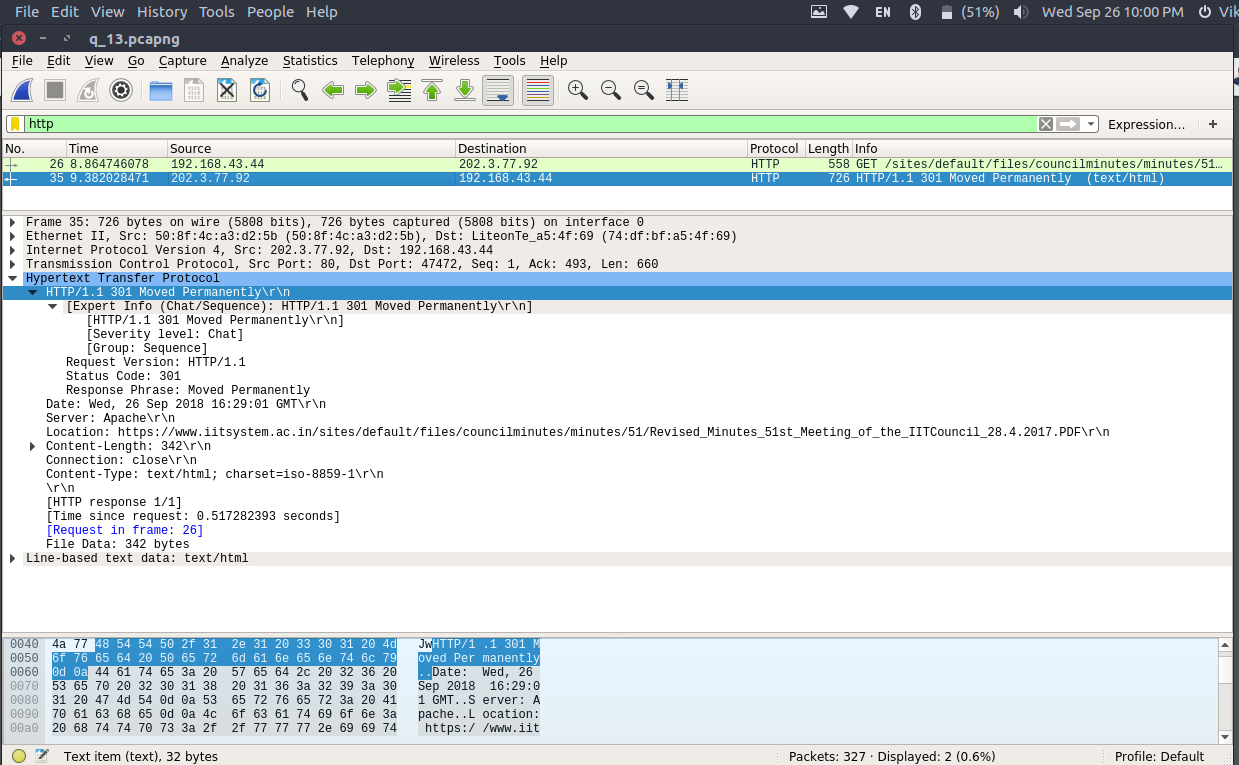
\includegraphics[scale=0.40]{1_13}
    \vspace{1cm}

    \noindent
    \textbf{\large Question 14}
    Note the time required to access the files viz.  simple1.html, simple2.html, simple3.html also and preparea table that shows the time required to access each of the files simple1.html, simple2.html, simple3.html,
    the pdf files in Q13 and the html file about counties in US, in question in section 3 that follows.\\
    \textbf{\large Answer}
    % 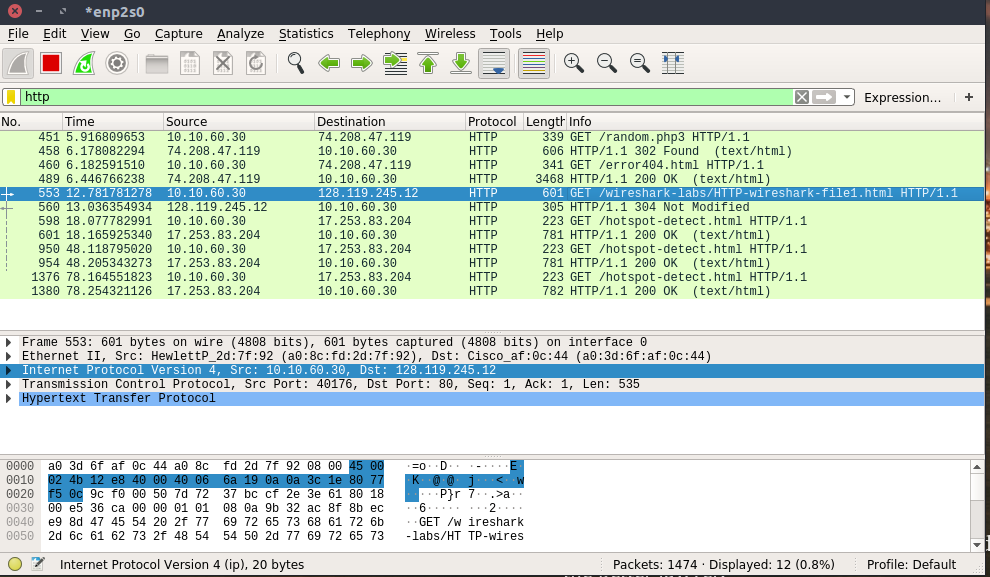
\includegraphics[scale=0.48]{2}
    \vspace{1cm}


    \begin{center}
        {\large \textbf{SET 2: The HTTP CONDITIONAL GET/response interaction }}
    \end{center}

    \noindent
    \textbf{\large Question 1}
    Inspect the contents of the first HTTP GET request from your browser to the server.
    Do you see an IF-MODIFIED-SINCE line in the HTTP GET?\\
    \textbf{\large Answer}
    No, ther is no IF-MODIFIED-SINCE line in HTTP GET from my browser to the server.\\[10pt]
    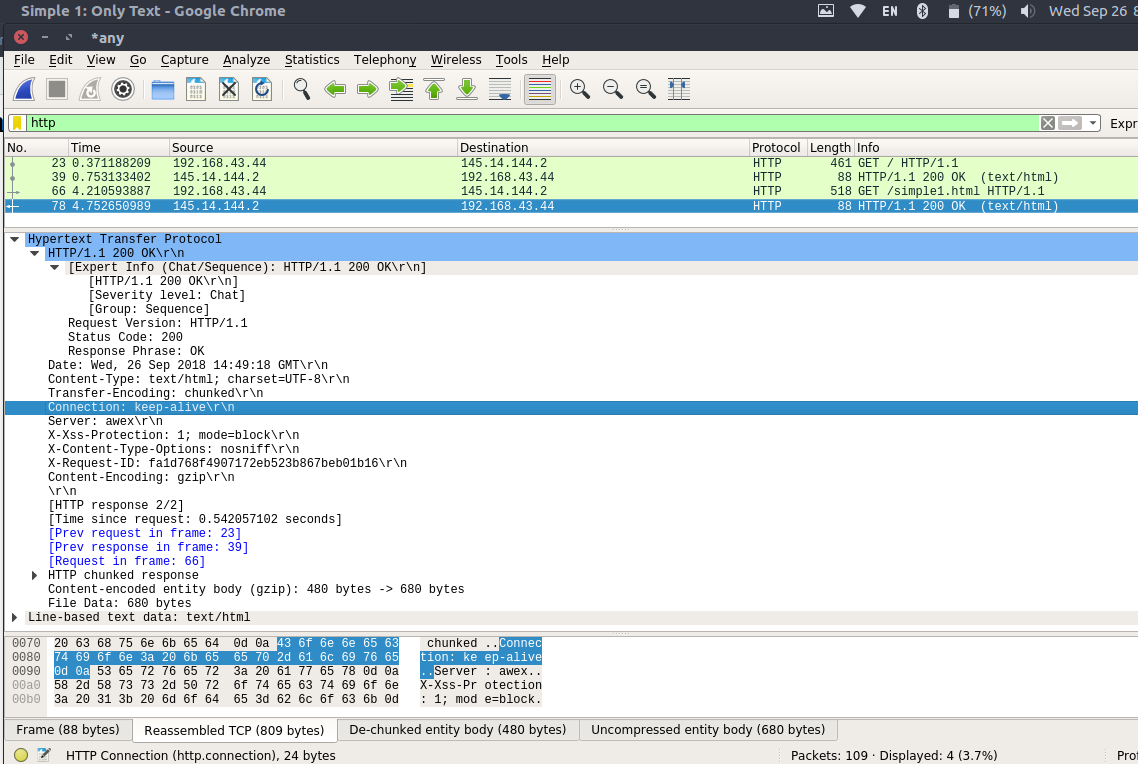
\includegraphics[scale=0.40]{1_2}
    \vspace{1cm}

    \noindent
    \textbf{\large Question 2}
    Inspect the contents of the server response. Did the server explicitly return the contents of the file?
    How can you tell?\\
    \textbf{\large Answer}
    Here is text returned in response of get method in the (Line Based text):\\[10pt]
    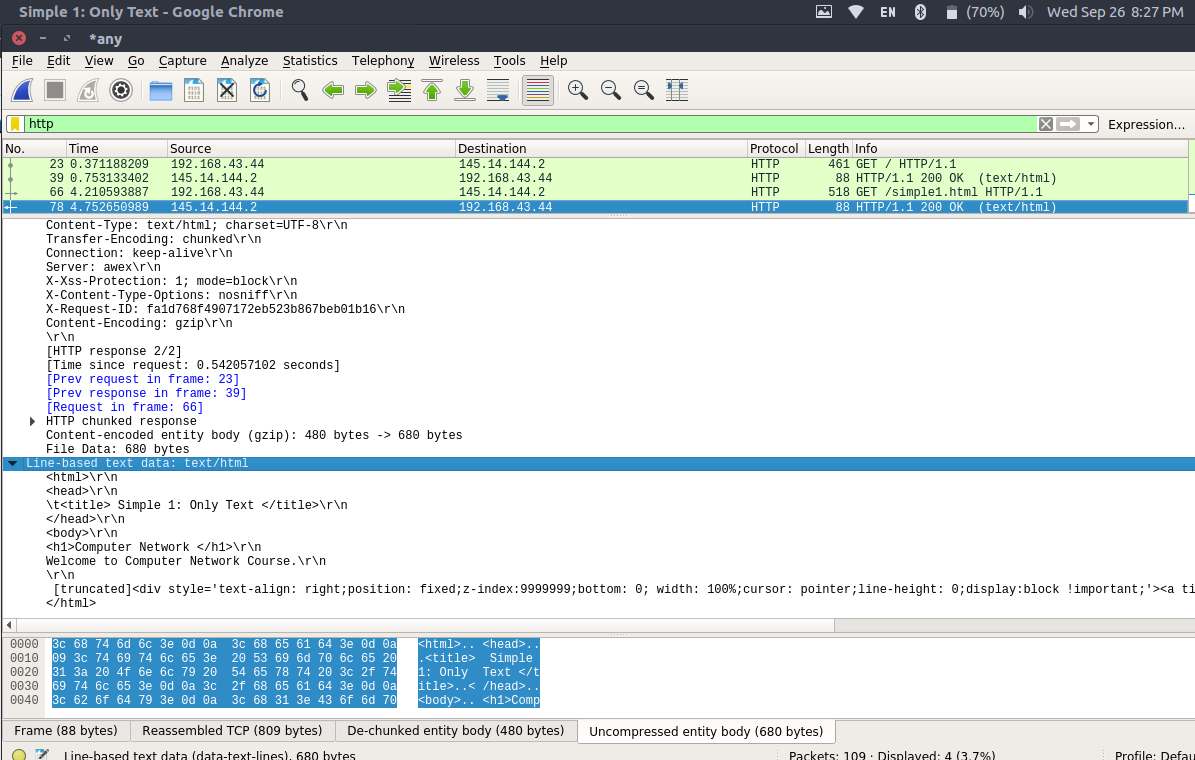
\includegraphics[scale=0.40]{1_3}
    \vspace{1cm}

    \noindent
    \textbf{\large Question 3}
    Now inspect the contents of the second HTTP GET request from your browser to the server.
    Do you seean IF-MODIFIED-SINCE: line in the HTTP GET? 
    If so, what information follows the IF-MODIFIED-SINCE: header?\\
    \textbf{\large Answer}
    No, Second get request doesn't has IF-MODIFIED-SINCE.\\[10pt]
    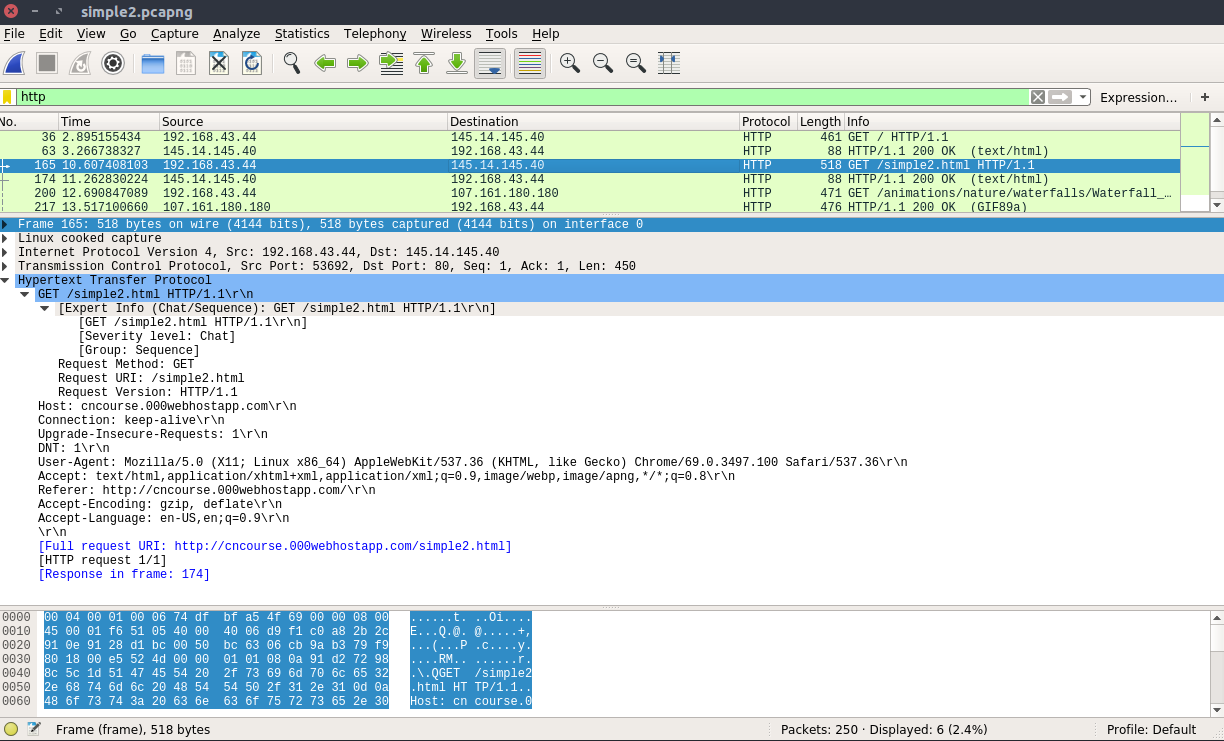
\includegraphics[scale=0.40]{1_10_1}\\[10pt]
    \vspace{1cm}

    \noindent
    \textbf{\large Question 4}
    What is the HTTP status code and phrase returned from the server in response to this second HTTP GET? 
    Did the server explicitly return the contents of the file?  Explain.\\
    \textbf{\large Answer}
    HTTP status code is 200 and the content is returned in response from the server.\\[10pt]
    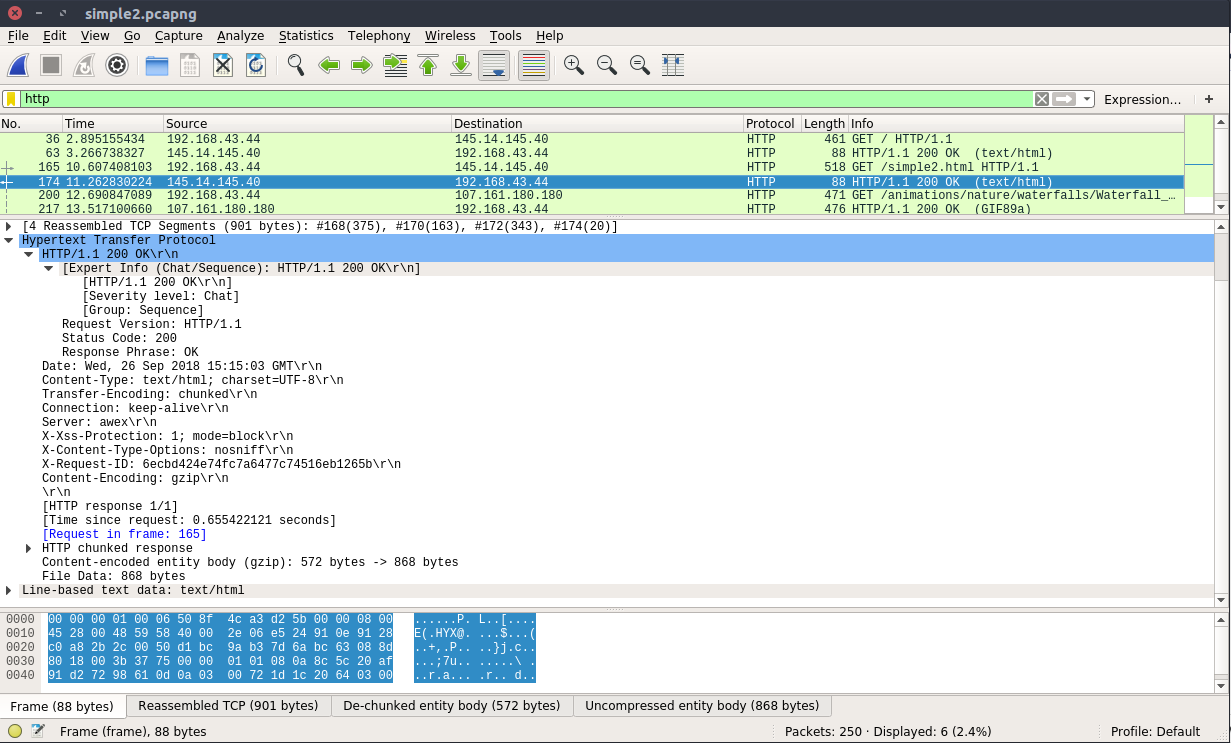
\includegraphics[scale=0.40]{1_10_2}\\[10pt]
    \vspace{1cm}

    \begin{center}
        {\large \textbf{SET 3: Retrieving Long Documents }}
    \end{center}

    \noindent
    \textbf{\large Question 1}
    How  many  HTTP  GET  request  messages  did  your  browser  send? 
    Which  packet  number  in  the  tracecontains the GET message ?\\
    \textbf{\large Answer}
    6 requests has been send by my browser totally for pdf and html file from which 1 for pdf and 1 for html file. Packet number 31 for 'Large Text' and 421 for 'pdf file'.\\[10pt]
    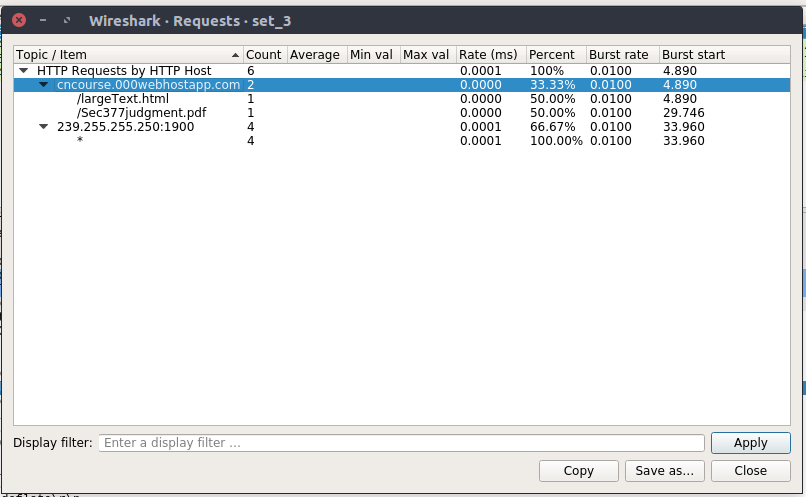
\includegraphics[scale=0.48]{s3_1}\\[10pt]
    \vspace{1cm}

    \noindent
    \textbf{\large Question 2}
    Which packet number in the trace contains the status code
     and phrase associated with the response to the HTTP GET request?\\
    \textbf{\large Answer}
    Packet number 305 for 'Large Text' (html file) and Packet number 3926 for 'pdf file'.\\[10pt]
    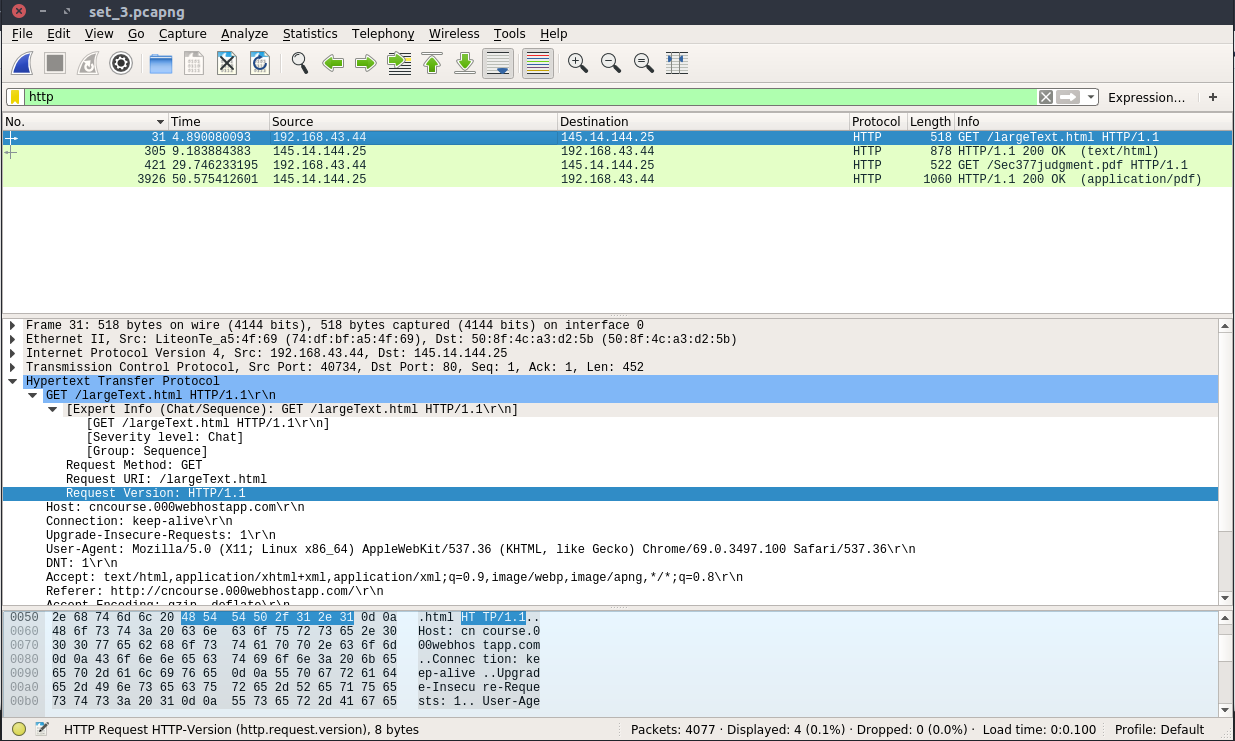
\includegraphics[scale=0.40]{s3}\\[10pt]
    \vspace{1cm}

    \noindent
    \textbf{\large Question 3}
    What is the status code and phrase in the response?\\
    \textbf{\large Answer}
    Status Code 200 for both html file and pdf file.\\[10pt]
    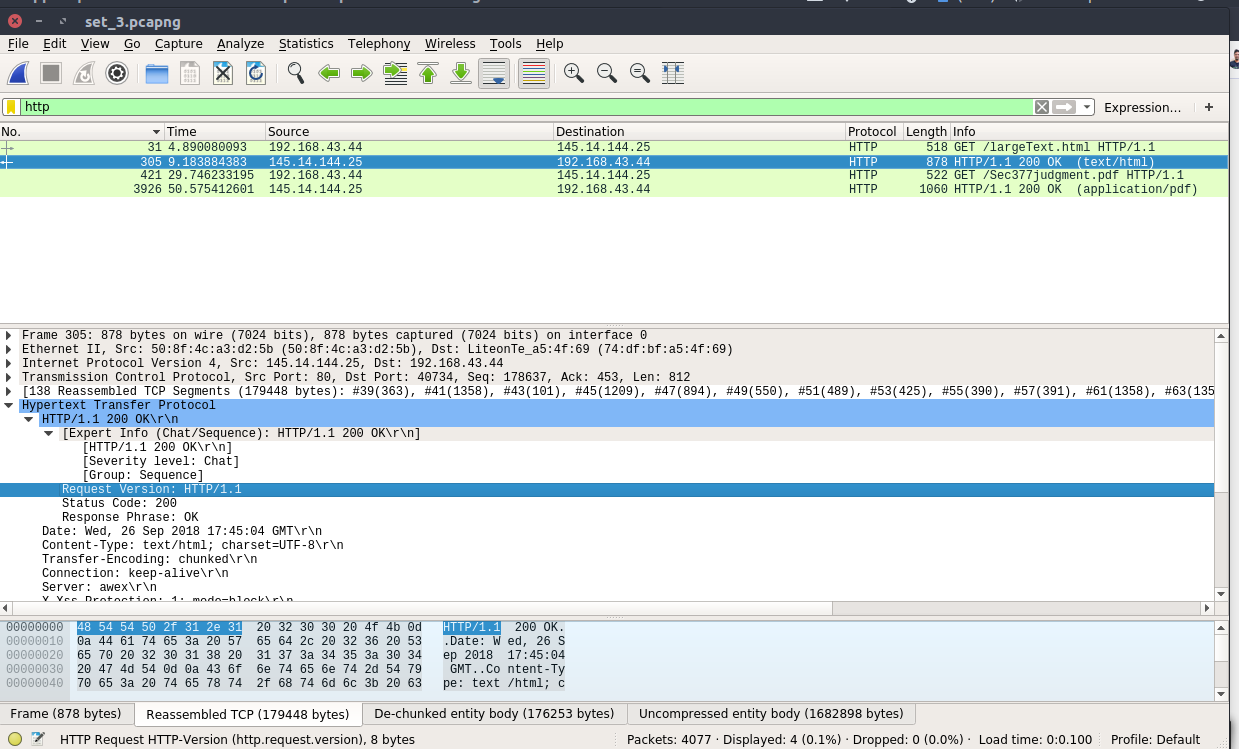
\includegraphics[scale=0.40]{s3_2}\\[30pt]
    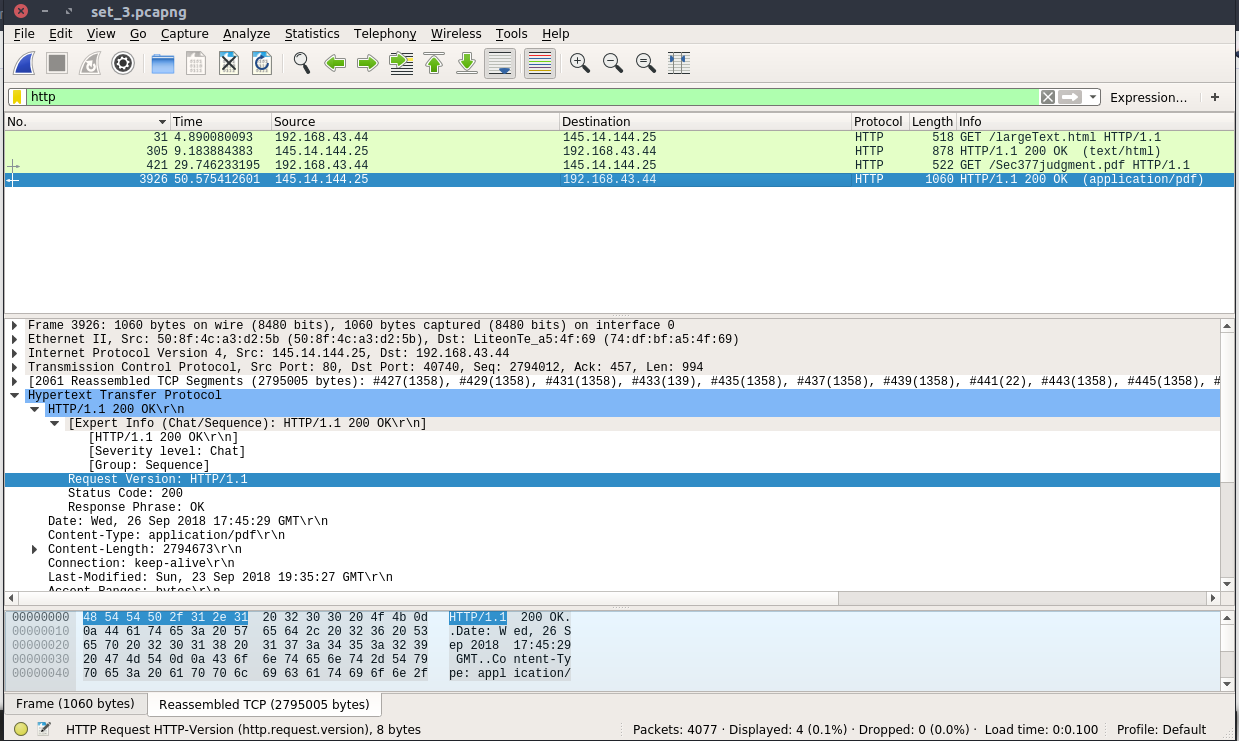
\includegraphics[scale=0.40]{s3_3}\\[10pt]
    \vspace{1cm}
    
    \noindent
    \textbf{\large Question 4}
    How many data-containing TCP segments were needed to carry the single HTTP response and the textof the file ?\\
    \textbf{\large Answer}
    138 TCP segments for html file and 2061 TCP segments for pdf file. Snapshots in last questions.
    \vspace{1cm}

    \begin{center}
        {\large \textbf{SET 4 - HTML Documents with CGI Script }}
    \end{center}
    
    \noindent
    \textbf{\large Question 1}
    What is the method used in your HTTP message ?  How many HTTP request messages did your browsersend?  To which Internet addresses were these requests sent?\\
    \textbf{\large Answer}
    POST method is used in HTTP message. 2 requests has been send by browser. To http://cncourse.000webhostapp.com/simple5.php.\\[10pt]
    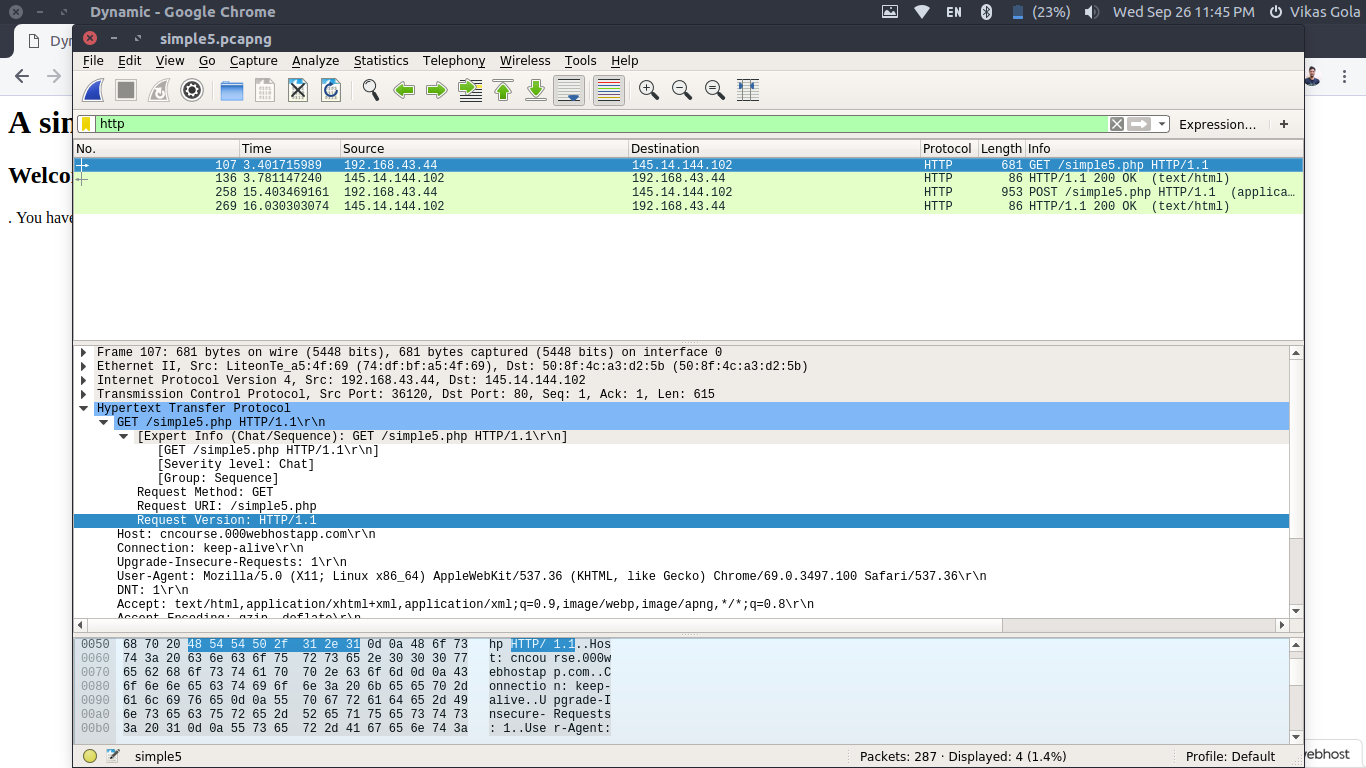
\includegraphics[scale=0.40]{s4}\\[10pt]    
    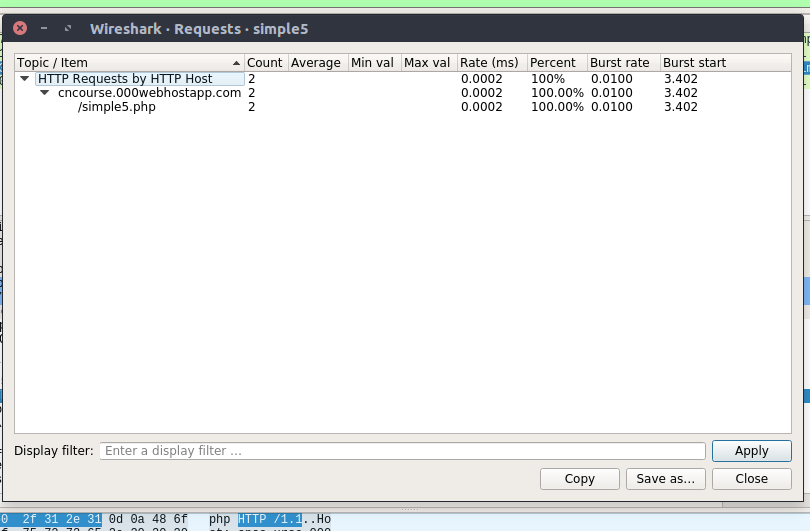
\includegraphics[scale=0.40]{s4_1}\\[10pt]    
    \vspace{1cm}

\end{document}